% ===========================================================================
\chapter{The Way to Write Katakana}\jchap{片仮名の書き方}
% [o] LABEL
\label{chap:TheWayToWriteKatakana}
\label{sec:TheWayToWriteKatakana}  % ifor dest
\label{sec:Gojuonzu}               % ifor dest
% [o] DESTINATIONS
\ifor{The Way To Write Katakana}{片仮名の書き方}{かたかな・の・かきかた}{Katakana Schreibweise}
\ifor{Gojūonzu}{五十音図}{ごじゅうおんず}{50 Laute Tafel}
% [o] INDEX
\ifor{mora}{モーラ}{もーら}{Mora}
\ifor{space character}{空白文字}{くうはく・もじ}{Leerzeichen}
\ien{Writing katakana}

The second\footnote{The first is Hiragana} Japanese Kana script a
\hyperref[sec:Mora]{mora}  based writing system is called Katakana and this is
written in Japanese as {片仮名} {【かたかな】} but sometimes also as
{カタカナ}.  It consists of a little less the 50 letters, as it is usual for
morae or \hyperref[sec:Syllable]{syllable} based systems. Katakana derived from
Chinese characters, called Kanji ( {漢字} {【かんじ】} in Japanese). All
Katakana together form a complete phonetic script.

\ifor{Gojūonzu}{五十音図}{ごじゅうおんず}{50 Laute Tafel}
The collection of Katakana is usually displayed in the Gojūonzu (lit. Table of
Fifty Sounds), a grid of 10x5 in which the characters are displayed. Even
though nominally the Gojūonzu is containing 50 characters the grid is not
completely occupied. Additionally there is also one character added to the
end. So with five gabs and one extra letter, the current number of Katakana is
46. If we would count also the character for doubling a vowel (which is not
displayed in the Gojūonzu) we have 47 distinct characters, still below 50. 

% アイウエオ
% カキクケコ
% サシスセソ
% タチツテト
% ナニヌネノ
% ハヒフヘホ
% マミムメモ
% ヤユヨ
% ラリルレロ
% ワヲ
% ン
\index{Katakana Gojūonzu}
\index{Katakana}
\index{Gojūon}
\index{片仮名五十音図}
\bigskip
\begin{center}
%\Huge
\Padding
%\begin{tabular}{m{1.0cm}||m{1.0cm}|m{1.0cm}|m{1.0cm}|m{1.0cm}|m{1.0cm}|}
\begin{tabular}{r||c|c|c|c|c|}
             & \textbf{a}& \textbf{i}& \textbf{u}& \textbf{e}& \textbf{o}\\ \hline \hline
\textbf{-}&ア&イ&ウ&エ&オ\\\hline 
\textbf{k}&カ&キ&ク&ケ&コ\\\hline 
\textbf{s}&サ&シ&ス&セ&ソ\\\hline 
\textbf{t}&タ&チ&ツ&テ&ト\\\hline 
\textbf{n}&ナ&ニ&ヌ&ネ&ノ\\\hline 
\textbf{h}&ハ&ヒ&フ&ヘ&ホ\\\hline 
\textbf{m}&マ&ミ&ム&メ&モ\\\hline 
\textbf{y}&ヤ&  &ユ&  &ヨ\\\hline 
\textbf{r}&ラ&リ&ル&レ&ロ\\\hline 
\textbf{w}&ワ&  &  &  &ヲ\\\hline 
\textbf{*}&ン&  &  &  &  \\\hline 
\end{tabular}
\end{center}



\ifor{space character}{空白文字}{くうはく・もじ}{Leerzeichen}
\ifor{homophone}{同音異語}{どうおん・いご}{Homophon}
\ija{同音語}
Even though Katakana can be used by its own to express the complete content of
the Japanese language it is almost never used as such. This is due to the fact
that the other two scripts Hiragana and Kanji exists and that there was
traditionally no space character to separate words. So a Katakana sentence with
Katakana only and no spaces is hardly understandable also due to many
homophones.  But even if there are spaced it is difficult. Therefore the letter
type boundaries of Kanji, Hirangana and Katakana are the most significant
indicator for word boundaries.

\ithree{role}{作用}{Funktion}\ide{Rolle}
In the Japanese\footnote{Until the end of World War II Katakana was used
differently. Official documents used a mix of Kanji and Katakana in a similar
way then Hiragana and Kanji today. Katakana was used for Particles and
Okurigana.} written language Katakana has a distinct role. It serves for:

\bigskip

\begin{tabular}{rp{15cm}}
1.& writing words of foreign origin\\
2.& words that need to be emphasized\\
3. &often indicate on-yomi in dictionaries\\
4.& names of minerals \\
5.& geological names \\
6.& names of fauna (animals)\\
7.& names of flora (plants)\\
8.& partly onomatopoeias in Manga\\
9.& sounds, like animal sounds or sounds made by humans\\
10.& Telegrams (before 1988)\\
11.& banking system account names\\
12.& In literature (eg. Manga) words being spoken in a (foreign) accent or "robotic" speech\\
13. &sometimes used as Furigana\\
14. & uncommon Kanji, eg.  {皮膚科} {【ひふか】} "dermatologist" written as {皮フ科}\\
15.& computer output (in 80th, before introduction of multi byte characters)\\
16. &some personal names (especially female) (common in the past: eg. セツ (setsu))\\

\end{tabular}

\medskip

\ifor{manga}{漫画}{まんが}{Manga}
Therefore in commercials, Manga and literature describing foreign concepts
Katakana has a over proportional usage.

\section{Pronunciation and Intonation}

The pronunciation of Katakana is the same as for Hiragana. Therefore every
syllable, more precise every mora corresponds to a Katakana character and is
constructed as 'consonant' + 'vowel' with the exception of |n|. This system of
letter for each mora makes pronunciation absolutely clear with no ambiguities.
However the simplicity of Katakana does not mean that pronunciation in Japanese
is simple for English speakers as it is for Germans.  The rigid structure of
the fixed mora sound in Japanese creates the challenge of learning the proper
intonation and duration of Japanese pronunciation.

Almost each Japanese word can be chunked into morae of high and low pitch witch
is a crucial aspect of the spoken language. Compared to Chinese, Japanese
luckily have only two pitches: hi and low. Sometimes this difference can be
even important for the lexic. Homophones can have for example a difference in
pitch which make them distinguishable.  The intonation of high and low pitches
is a crucial aspect of the spoken language. One of the biggest problems for
obtaining a natural sounding pronunciation is the incorrect intonation. Many
European or American learners speak without paying attention to the correct
pitch. That makes the speech sound non-natural for Japanese. In some language
course try to let the learner memorize the natural pitch of a word or even
teach rules for memorization. While there is clearly a possibility for
linguistic rules, they are hard to remember and master. Also because they can
remember the rules it is still possible to learn the correct intonation by
resorting to language learning techniques used by infants or small children:
mimicking native Japanese speakers. Therefore it is highly advised to expose
oneself to as many Japanese spoken language as possible and to mimic it. Radio,
podcasts, drama and television to name a few. However, it is not advised to
listen too much artificial sources like anime or commercials.

\bigskip
\begin{tabular}{rl}
-&every (yes \textbf{every}) mora is pronounced with the same length\\
-&there is no short and long mora or letters\\
-&every mora has a pitch: high or low\\
-&every pitch matters\\
-&the pitch can change  sometimes with its context\\
-&the pitch can change with a dialect - however standard Japanese has well defined pitches\\
\end{tabular}

\bigskip
The pronunciation of Katakana is exactly the same as for Hiragana and most
sounds are very close to the Latin pronunciation but in general are pronounced a
little shorter without any stress. Only the /ra/ sounds, like in /ra/, /ri/, /ru/,
/re/ and /ro/ have no similarity in European languages. 


The sound of the Japanese /r/ is  neither a central nor a lateral flap, but may
vary between the two. To an English speaker, its pronunciation varies between a
flapped 'd' (as in American English buddy) and a flapped 'l'.
\href{http://en.wikipedia.org/wiki/Japanese_phonology}{(Wikipedia Japanese
Phonology)}.


The following table displays the pronunciation in the Gojūonzu.

\ien{Rōmaji Gojūonzu}
\ien{Rōmaji}
\ien{Gojūon}
\ija{ローマ字五十音図}
\ija{ローマ字}
\bigskip
\begin{center}
%\LARGE
%\Huge
\Padding
\begin{tabular}{c||c|c|c|c|c|}
&\textbf{a}&\textbf{i}&\textbf{u}&\textbf{e}&\textbf{o}\\\hline\hline
\textbf{-}&a&i&u&e&o\\\hline
\textbf{k}&ka&ki&ku&ke&ko\\\hline
\textbf{s}&sa&shi&su&se&so\\\hline
\textbf{t}&ta&chi&tsu&te&to\\\hline
\textbf{n}&na&ni&nu&ne&no\\\hline
\textbf{h}&ha&hi&fu&he&ho\\\hline
\textbf{m}&ma&mi&mu&me&mo\\\hline
\textbf{y}&ya&&yu&&yo\\\hline
\textbf{r}&ra&ri&ru&re&ro\\\hline
\textbf{w}&wa&&&&o\\\hline
\textbf{{*}}&n&&&&\\\hline
\end{tabular}
\end{center}





\section{Writing Katakana Letters - 片仮名を一つづつ書く} \label{sec:WritingKatakanaLetters}

Writing Katakana words start with writing single Katakana letters. Knowing the
writing and reading of Katakana letters is essential to pronounce foreign words
in Japanese correctly. And that is even more important for learners who have
good English knowledge, because it is very tempting to pronounce English words
in Japanese with original English pronunciation, which is seldom
understood\footnote{The reader might try to order a cheeseburger at a fast food
restaurant insted of a /chiizubaagaa/ (チーズバーガー).} by Japanese people
who are used to their Japanese-English pronunciation. 

By learning Katakana the understanding of morae and syllables will also 
help to improve the pronunciation and understanding of Japanese. 

Katakana as most letters are a joint combination of strokes. For the writing of Katakana
some rules are important, which are presented here out of order.


\begin{description}

\item[Order:] The order of strokes is important. In section
\ref{sec:StrokeOrderMatter} on page \pageref{sec:StrokeOrderMatter} more can be found. 

\item[Fasted Method of Writing:] Often the fastest possible method of writing
or order of strokes is the correct one.  Often from left upper corner to right
lower corner. But exceptions do exist.

\item[The characters (letters) are \textit{not} symmetric.]

\item[All characters (letters) occupy a square.]

\item[The aesthetic:] What make the character to a beautiful character? The
answer is different for each character.

Following some possibilities of rule generation for the character ``u''
 {「ウ」 }:

\bigskip \CharacterExplanation{u-guide2}{The most important feature is that the
second and third line do not align. This is not an accident.}

\bigskip \CharacterExplanation{u-guide0}{Except many Hiragana for some Katakana
the base line is aligned with horizon. As with this character. }


\bigskip \CharacterExplanation{u-guide1}{Also the start (or turning) points of
all other lines are aligned vertically. Which gives this Katakana its unique
square look.}


\bigskip \CharacterExplanation{u-guide}{All together some lines need to be
remembered to write the letter beautiful.}

\bigskip

\item[A different logic:] A little bit less the Hiragana, but also in Katakana
there are some lines that do not align horizontally  or vertically. Or to say
it differently some characters are not stright on purpose.

\end{description}

On top of this the following is most likely valid: Only if one can write a
letter it is (easier) possible to faster learn and memorize it.


%----------------------------------------------------------------------------
\subsection{Stroke Order Matter! - 書き順事項}\label{sec:StrokeOrderMatter}

Some European individualists might ask them self \textit{"Why do I have to
remember the order of strokes - I don't obay this in my language - and who
defined this in the first place (if not me)?"} and this seems obvious in
Europe. However some reason for order exist. 

% 書き順事項 【かきじゅんじこう】

\begin{description}

\item[1. Impression:] It make a unprofessional impression to Japanese, if one
writes characters in the wrong order. Some laughs can be observed at least.

\item[2. Tests:]  In some tests/ exams (in Japan) the order of strokes will be
tested and one got 0 points for the wrong order. 

\item[3. Time Savings:] In the most cases the predefined order is the fastest
way to write a character. Overall once save (life) time.

\item[4. Readability:] In some cases characters become readable only (or
beautiful) of the order is correct.

\item[5. Confusion Danger:] For only some characters the order is utmost
important. If not obeyed it is very likely (almost certain) that this
characters become a candidate for a wrong interpretation. 

\end{description}
\normalsize

\newpage
%----------------------------------------------------------------------------
\subsection{Example /u/  - {「ウ」の例} }

The Katakana /u/ is written as {「ウ」} in Japanese. The character is composed
out of the following three components:

\bigskip 
\CharacterExplanation{uds1}{This is stroke 1}
\bigskip 
\CharacterExplanation{uds2}{This is stroke 2}
\bigskip 
\CharacterExplanation{uds3}{This is stroke 3} 

Of course the strokes need to be at the right place. So better always think or draw 
a frame aound. Or even better write the strokes into a frame from the beginning!

\bigskip 
\CharacterExplanation{udss1}{This is stroke 1 in a square frame}
\bigskip 
\CharacterExplanation{udss2}{This is stroke 2 in a square frame}
\bigskip 
\CharacterExplanation{udss3}{This is stroke 3 in a square frame} 


%\begin{center}
%\textbf{Stroke 1:} 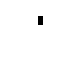
\includegraphics[trim= 00 15 00 00]{../share/katakana/uds1.pdf}
%\textbf{Stroke 2:} 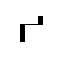
\includegraphics[trim= 00 15 00 00]{../share/katakana/uds2.pdf}
%\textbf{Stroke 3:} 
\includegraphics[trim= 00 15 00 00]{../share/katakana/uds3.pdf}
%\end{center}
\bigskip

This components have to be written in the above mentioned enumeration order one
after another. (The first example is without frame)

\bigskip 
\CharacterExplanation{udg1}{This is stroke 1 in context}
\bigskip 
\CharacterExplanation{udg2}{This is stroke 2 in context}
\bigskip 
\CharacterExplanation{udg3}{This is stroke 3 in context}

%\begin{center}
%\textbf{Stroke 1:} 
\includegraphics[trim= 00 15 00 00]{../share/katakana/udg1.pdf}
%
%\textbf{Stroke 2:} 
\includegraphics[trim= 00 15 00 00]{../share/katakana/udg2.pdf}
%
%\textbf{Stroke 3:} 
\includegraphics[trim= 00 15 00 00]{../share/katakana/udg3.pdf}
%\end{center}

\bigskip 
\CharacterExplanation{udgs1}{This is stroke 1 in context in a square frame}
\bigskip 
\CharacterExplanation{udgs2}{This is stroke 2 in context in a square frame}
\bigskip 
\CharacterExplanation{udgs3}{This is stroke 3 in context in a square frame}

\bigskip

In the Katakana training section in this document the order will be introduced
as red numbers and arrows which give the approximate direction where to place
the writing device. 

%\begin{center}
% 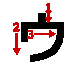
\includegraphics[trim= 00 05 00 00]{../share/katakana/us.pdf}
%\end{center}
\bigskip

\CharacterExplanation{us}{Write the first short strokes straight from up to
down. Then - and this is difficult place the second stroke in the correct
distance from the first one. Luckily this is also a straight stroke from up to
down. }

\bigskip

Of course the perception changes if the character is written in a square.
Remember that it is better to write the character in a square, because the
correct spaces between the character and the frame also determinates its
beauty.

\bigskip

\CharacterExplanation{uss}{The first stroke in the frame is not difficult as
mentioned before from straight up to down. However the frame helps because now
we understood that it is centered. The second stroke become also easier in a
frame because it is written at the edge of the character. After some time and
experience this is better understood. The last stroke has to join the first and
second stroke. That is still difficult with or without a frame.}

\bigskip

%----------------------------------------------------------------------------
\subsection{Stroke Types - 筆画の種類}

In European language there is no idea to have different stroke types unless one
enter the field of calligraphy. In Japanese there are different kind of
strokes.  Most important for Kanji, second important for Hiragana and least
important for Katakana since Katakana is also used for a bold replacement.  Due
to this fact the five different type of Japanese strokes ({筆画の種類}
{【ひっかくのしゅるい】}) will not repeated here. For now it is perfectly fine
to make all strokes equally thick. 



%\input{../share/sec/WritingKatakanaSentences}
\section{Special Katakana Characters}\jsec{特別カタカナ}
% [o] LABEL
\label{sec:SpecialKatakanaCharacters}
% [o] INDEX
\ifor{special Katakana characters}{特別カタカナ}{とくべつかたかな}{Spezielle Katakana Zeichen}
\ifor{Katakana}{片仮名}{かたかな}{Katakana}
\ifor{Gojūonzu}{五十音図}{ごじゅうおんず}{50 Laute Tafel}


As mentioned before \hyperref[sec:Katakana]{Katakana} is almost like Hiragana.
This is true for the \hyperref[sec:Gojuonzu]{Gojūonzu (50 sound table)  {五十音図}
{【ごじゅうおんず】}} This section will show the special characters, some are
different from the Hiragana set.

Special in some sense are characters used for punctuation, like {「。」},
{「!」} and {「?」}.  These are similar to the western counterparts but
differ a little bit. While it is obvious for the small circle {「。」}, also
{「!」} and {「?」} differ from the western equivalent in that sense that
they are \textbf{centerd} and occupy more (white) space. This characters among
other characters are used equally among Hiragana,
\hyperref[sec:Katakana]{Katakana} and Kanji. Therefore this section will not
further mention them.

%TODO check if point changes orientation and alignment in case of changing
%writing direction. 

\subsection{Doubling Vowels in Katakana}\jsubsec{カタカナでの倍増母音}
% [o] LABEL
\label{subsec:DoublingVowelsInKatakana}
\label{subsec:DoublingVowels}
\label{sec:DoublingVowelsInKatakana}
\label{sec:DoublingVowels}
% [o] INDEX
\ifor{doubling vowels}{倍増母音}{ばいぞうぼいん}{Vokalverdopplung}
\ifor{repition mark}{繰り返し記号}{くりかえしきごう}{Wiederholungszeichen}
\ifor{Katakana}{片仮名}{かたかな}{Katakana}

% カタカナでの倍増母音 【ばいぞうぼいん】

Special \hyperref[sec:Katakana]{Katakana} characters do also exists. The most
important character is Chōon {長音} {【ちょうおん】} the plain iteration
character {「ー」}, written as a stroke. It is one of the very few which
changes orientation according the writing orientation. When writing
\hyperref[sec:Katakana]{Katakana} from left to right the iteration character is
horizontal, while writing \hyperref[sec:Katakana]{Katakana} from up to down it
is vertical. The function of this character is to double the previous mora.
This is also different from Hiragana. (For doubling als other
\hyperref[sec:Katakana]{Katakana} caracter, refere to section
\nameref{sec:Iteration} on page \pageref{sec:Iteration}.)

\bigskip

\CharacterExplanation{k-iteration-s}{In standard gothic fonts the
\hyperref[sec:Katakana]{Katakana} iteration character is just a straight line
and it is not possible to understand in which direction it has to written. }

\bigskip

\CharacterExplanation{k-iteration-sm}{However if it is written with a different
font or with a brush it is clearly visible that in horizontal writing it is
written from left to right.} 

\bigskip


%\definecolor{orange}{rgb}{1,0.5,0}
%\definecolor{mygreen}{rgb}{.2,1,.2}

\bigskip
\textit{Example:}

\bigskip

\begin{center}
\begin{tabular}{p{7cm}p{7cm}}
Katakana:&Hiragana:\\
\Huge カ\textbf{\color{magenta}ー}ド /kaado/ &\Huge か\textbf{\color{magenta}あ}ど /kaado/\\
\end{tabular}
\end{center}

\bigskip

This character is very often used and makes \hyperref[sec:Katakana]{Katakana}
for this easier then Hiragana. The long vowel ambiguity do not exist.

As mentioned above the orientation of the \hyperref[sec:Katakana]{Katakana}
iteration character changes with the direction of writing. The above example
with different writing orientation.

\medskip
\textit{Example:}

\medskip

\begin{center}
\begin{tabular}{p{3.5cm}p{3.5cm}p{3.5cm}m{3.5cm}}
horizontally&
\setCJKfamilyfont{cjk-vert}[Script=CJK,RawFeature=horizontal]{IPAPGothic}
\mbox{
\begin{minipage}{3.2cm}
\Huge カ\textbf{\color{magenta}ー}ド
\end{minipage}
}
& vertically &
%\setCJKfamilyfont{cjk-vert}[Script=CJK,RawFeature=vertical]{Kozuka Gothic Pro M}
\setCJKfamilyfont{cjk-vert}[Script=CJK,RawFeature=vertical]{IPAPGothic}
\raisebox{-.5\height}{
\mbox{
\rotatebox{-90}{
\begin{minipage}{3.2cm} \CJKfamily{cjk-vert}
\Huge カ\textbf{\color{magenta}ー}ド
\end{minipage}
}
}
}
\\
\end{tabular}
\end{center}
\medskip



\subsection{Seldom Used Katakana}\jsubsec{めったに使われない片仮名}\label{subsec:SeldomlyUsedKatakana}

% めったに使われない片仮名 【めったにつかわれないかたかな】

Even though |wo| {「ヲ」}  is part if the standard letters. But since all
particle are written in Hiragana and in this case |wo| is written {「を」} the
learning of {「ヲ」} can be skipped. Unless it is important to read old texts,
like telegrams.



